%!TEX root = ../main.tex

\chapter{太陽光発電による電力グリッドシステム}
\section{電力グリッドの概要}
電力グリッド(電力系統，Electrical grid)とは，発電した電力を電力を必要とする設備に供給するために，発電・変電・送電・配電・充放電の各工程を統合したシステムである．

\section{本研究で扱う対象}
本研究では高知県の某工場を対象とする．本研究の対象は以下の要素で構成されている．
\begin{itemize}
	\item 電力の導線
	\item 太陽光発電設備\\
	工場屋上に設置された発電設備．
	\item 電力消費機器\\
	空調照明，および製造用機械など，電力を消費する設備群．本研究の対象では設備群が3つ存在する．
	\item 蓄電池\\
	電力量の需給調整や非常用電源として機能する設備．
	\item 電力変換装置\\
	パワーコンディショナや変圧器などの，電圧を変換したり，交流から直流，あるいはその逆に変換する設備.
	\item 商用電力系統\\
	卸売電力取引所や電力会社から電力を購入・受電したり，電力を売電するために接続されている外部系統． 
	電力を購入するにあたり，単位電力量あたりの料金単価は市場価格に応じて変動する． 
	また，連続する30分間の平均使用電力を需要電力とし，
	その月の最大需要電力と過去11ヶ月の最大需要電力のうち，大きい方の値を基準に契約電力が決定され，契約電力に応じて基本料金が課される．\cite{m}
	\item 自己託送先\\
	自社で発電した余剰電力を，外部のネットワークを介して送電する設備群．
	\item 余剰電力の破棄先\\
	発電した電力が需要や蓄電容量，および売電可能量を超過した場合に，
	余剰分を破棄するための仮想的な領域．
	数理モデル上では電力の破棄として扱われるが，物理的にはパワーコンディショナの出力制御機能による発電量の抑制に相当する．	
\end{itemize}
	
本研究における電力運用の大きな特徴は，構成要素に太陽光発電設備と蓄電システムが含まれている点，
および商用電力系統からの買電単価が市場に応じて変動する点にある．%また，余剰電力を自己託送する要求が存在する点も特徴的である．
したがって，将来の予測発電量や予測消費電力量，予測料金単価%，および自己託送先の需要予測値
を踏まえつつ，
いかなるタイミングでどの程度の電力を蓄電池に充放電させるかを決定することが肝要となる．本研究で扱う対象を図\ref{fig:tecseed}に示す．
\begin{figure}[h]
	\centering
 	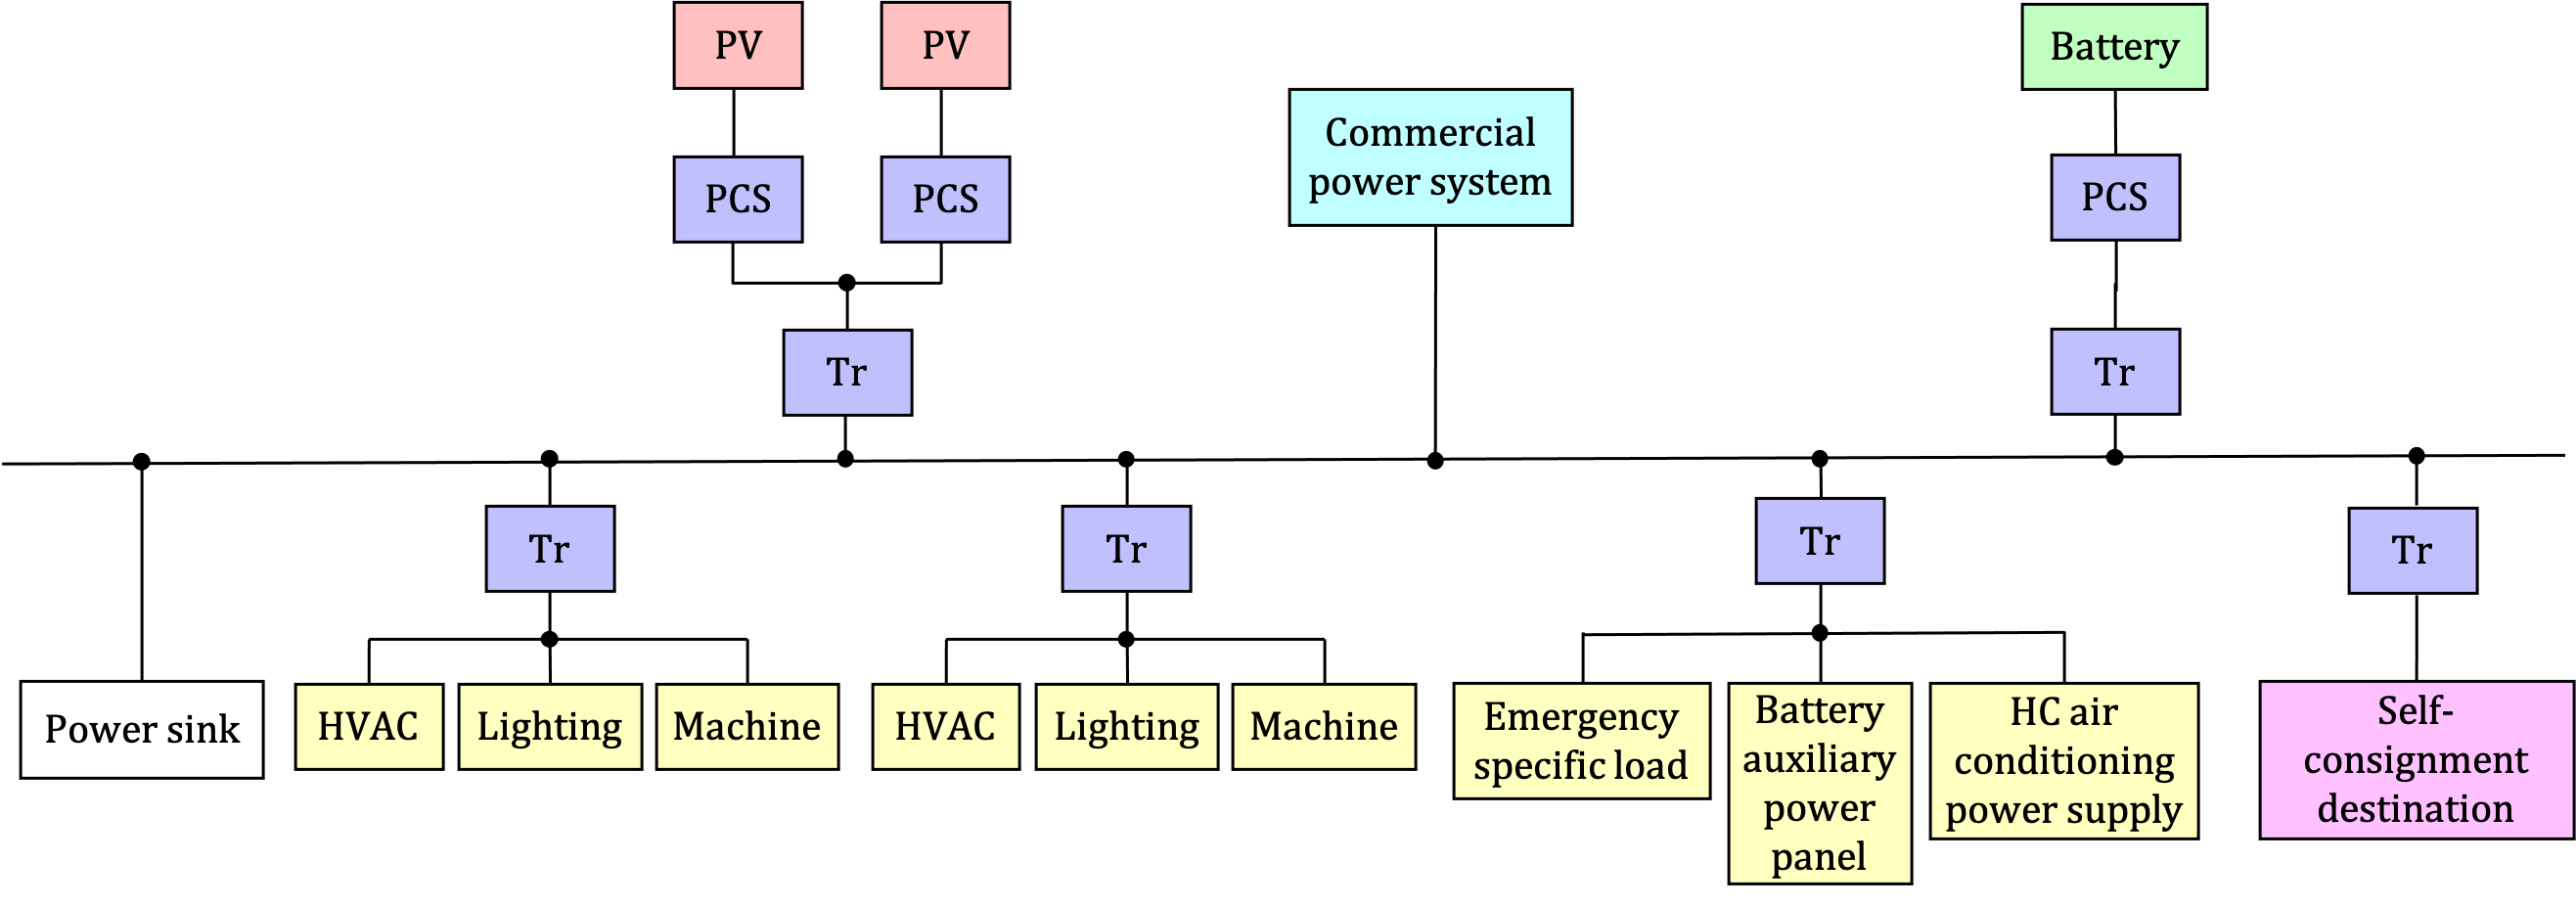
\includegraphics[width=215mm ,angle=270]{../figure/food_techno_eng.png}
 	\caption{Architecture of target system(PV: Photovoltaic, PCS: Power Conditioning System, Tr: Transformer)}
 	\label{fig:tecseed}
\end{figure}

\section{本研究で扱う対象が満たすべき事項}\label{sec:object}
本研究で扱う電力グリッドをモデル化するにあたり，考慮すべき事項を，モデル構築の基礎となる前提条件，設備や運用ルールに基づく制約条件，および最適化によって達成を目指す運用目的上の条件の3つに分類して定義する．

\subsection{モデル化における前提条件}
本研究の数理モデルにおいて，物理的な整合性を保つために導入する仮定である．
\begin{itemize}
	\item 導線\\
	導線の各接続点において，流入する電力と流出する電力の総和が等しいものとする．
	\item 電力変換装置 \\
	パワーコンディショナや変圧器などを介して電力を変換・送電する際，一定の変換効率に応じた電力損失が発生するものとする．
\end{itemize}

\subsection{システムおよび運用上の制約条件}\label{sec:object_seiyaku}
各設備の仕様および，電力契約や制度上のルールとして遵守しなければならない事項である．
\begin{itemize}
	\item 蓄電池
	\begin{itemize}
		\item 蓄電池の残量は常に定められた範囲内を外れないこと．
		\item 単位時間あたりの充放電電力は，最大出力を超過しないこと．
	\end{itemize}
	\item 商用電力系統 \\
	任意の連続する30分間の区間について，商用電力系統からの総買電力を一定量以下に制限すること．
	\item 自己託送先 \\
	自己託送先の需要電力量を上回る送電を行わないこと．
\end{itemize}

\subsection{運用目的上の条件}
上記の制約条件を満たした実行可能領域の中で，最適化によって最大化・最小化を目指す評価指標である．
\begin{itemize}
	\item 商用電力系統 \\
	期間内の商用電力からの買電コストを最小化すること．
	\item 自己託送先 \\
	可能な限り多くの余剰電力を自己託送に回すこと．
\end{itemize}

